\documentclass[10pt,a4paper]{article}
\usepackage[utf8]{inputenc}
\usepackage[czech]{babel}
\usepackage[T1]{fontenc}
\usepackage{amsmath}
\usepackage{amsfonts}
\usepackage{amssymb}
\usepackage{graphicx}
\usepackage{titlesec}
\author{Vojtěch Hudeček}
\title{Pacmen program documentation}
\begin{document}
\begin{center}

\begin{LARGE}
\textbf{Zápočtový program - Pacmen }

\textbf{Vojtěch Hudeček}

\textbf{Letní semestr, ak. rok 2012/13}
\linebreak 
\chapter{Uživatelská dokumentace}
\end{LARGE}
\end{center}
\section{Úvod}
Hru Pacman vytvořil v roce 1980 pro japonskou společnost \textit{Namco} Toru Iwatani. Hra se stala kultovní a je známá dodnes.
Ve hře hráč ovládá postavičku Pacmana, která je uvezněna v bludišti s duchy, kteří ji pronásledují.
V bludišti je umístěno množství tabletek které hráč musí snist a vyhnout se kontaktu s duchem, nebo bude zabit. Když ovšem hráč sní speciální tabletu, může naopak duchy likvidovat on.
Hra Pacmen je variací této hry ve které, jak název napovídá, je možno zapojit více hráčů, kteří pak soupeří nejen s monstry v bludišti ale i mezi sebou.
\section{Pravidla hry}
\subsection{Hráči}
Hra je určena pro 1-4 hráče. Hráči jsou na začátku hry umístěni v rozích bludiště. Ovládání hráčů je neměnné, a je popsáno ve startovním rohu hráče. Jména hráčů jsou seřazena v pravé části okna.
\paragraph{ovládání hráče}
\begin{center}

\includegraphics[scale=0.7]{images/arrows.png}
\end{center}
\subsection{Pohyb}
Hráč se pohybuje setrvačně, to znamená, že pokud je uveden do pohybu, zastaví se až když narazí do stěny.
Hráč může měnit směr na křižovatkách a otočit se o 180$^{\circ}$ v uličce.
Monstra se pohybují stejným způsobem, obrátit se však mohou pouze na křižovatce.
Hráči i monstra se pohybují stejnou rychlostí. Výjimkou je pouze hráč v režimu boss, který se pohybuje rychleji (viz. dále)
Dalším prvkem hry jsou teleporty. Vstoupí-li hráč či mosntrum do teleportu, objeví se u druhého konce stejné barvy.
\paragraph{teleport}
\begin{center}
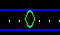
\includegraphics[scale=0.7]{images/port.png}
\end{center}
\subsection{Průběh hry}
Ve většině uliček v bludišti jsou tabletky, jejichž snědení přidá hráči bod. V některých bludištích jsou také červené kruhy představující oheň, které naopak bod uberou. Hráč dále může sníst speciální žlutou tabletu, která ho uvede dočasně do režimu boss. V tomto režimu hráč získá modrý kruh, je rychlejší, a může pojídat monstra. Je také chráněn od ostatních hráčů, na druhou stranou ani on jim není nebezpečný.
Hráči v režimu boss zmodrá jméno, a je vidět, kolik času zbývá.
\paragraph{ohnivé kruhy, boss mód}
\begin{center}
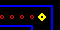
\includegraphics[scale=0.7]{images/example.png}

\includegraphics[scale=0.7]{images/boss.png}
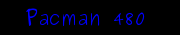
\includegraphics[scale=0.7]{images/boss_name.png}
\end{center}
\subsection{Kolize}
Dojde-li k dotyku hráče a monstra, mohou nastat dvě situace. Je-li hráč v režimu boss, zlikviduje monstrum a přičte si padesát bodů.
Monstrum se následně objeví na pozici k tomu určené. Je-li hráč v obyčejném režimu, je zabit a hra pro něj končí.
\\
Dojde-li ke kolizi dvou hráčů, je zabit ten, který má menší skóre. Pokud je jeden z hráčů v režimu boss nebo mají hráči stejné skóre, nestane se nic. Hráči poznají kdo má větší skóre při pohledu na pravou stranu okna a také podle barevných kruhů. Platí, že červený má více bodů než fialový a ten více než zelený. Hráč bez kruhu má nejméně bodů.
\paragraph{přičtení bodů, smrt Pacmana,kruhy}
\begin{center}
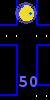
\includegraphics[scale=0.7]{images/plus_50.png}
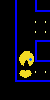
\includegraphics[scale=0.7]{images/pac_death.png}
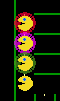
\includegraphics[scale=0.7]{images/party.png}
\end{center}
\section{Ovládání hry}
Hráči se ovládají pomocí 4 kláves zobrazených ve výchozím rohu hráče. Pro ovládní hry lze použít funkční klávesy popsané v horní části okna. Po stisku klávesy F10 nebo po skončení hry vstoupí hra do menu. Mezi jednotlivými položkami se naviguje pomocí kurzorových šipek.
V menu je možnost spustit novou hru, přidat či odebrat hráče či přejmenovat hráče. Při přejmenovávání je třeba pomocí klávesy Enter potvrdit všechna jména. V menu je také možné pomocí šipek doleva a doprava zvolit jinou mapu.
\pagebreak 
\paragraph{výchozí pozice monster}
\begin{center}
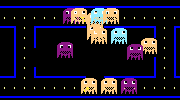
\includegraphics[scale=0.7]{images/monsters.png}
\end{center}
\section{Vyvtáření map}
Přidáním souboru se jménem map\_ číslo.txt do adresáře maps dojde k vyvoření nové mapy. Soubor musí obsahovat několik řádků v přesně určeném pořadí, a dále mapu o rozměrech 80 znaků na šířku a 60 na výšku. Mapa musí splňovat několik podmínek. Musí být ohraničena hvězdičkami, musí mít volné všechny 4 rohy a musí obsahovat nejméně jeden znak stříšky, což je výchozí pozice pro monstra. Zeď v mapě je označena hvězdičkou, tabletka podtržítkem, prázdné místo nulou, oheň minusem a brána teleportu číslem 1 - 9. Každý teleport musí mít 2 konce, a jeho číslo nesmí být vyšší než je počet barev uvedených na začátku souboru. Mapa by také měla obsahovat 4 velká P, což jsou počáteční umístění hráčů. Na začátku je také možné zvolit název přehrávané písně umístěné ve složce \textit{music} a barvu zdí. V případě, že nechceme hudební podklad, je místo jména písně uveden znak mřížky. Je vhodné použít soubor se šablonou mapy.
\end{document}
